\usetikzlibrary{math}

\newlength{\barwidth}
\setlength{\barwidth}{0.5cm}

\newcommand{\drawaxes}[1]{
  \draw [->] (-.2, 0) -> (4 * \barwidth + .2cm, 0) node[anchor=west] {$x$};
  \draw [->] (-.2, 0) -> (-.2, 5.2) node[anchor=south] {$#1$};
  \foreach \x in {0, ..., 4}
    \draw (\x * \barwidth, -1pt) -- (\x * \barwidth, 1pt);
  \foreach \x/\char in {0.5/$a$, 1.5/$b$, 2.5/$c$, 3.5/$d$}
    \draw (\x * \barwidth, 0) node[anchor=north, text height=8] {\char};
}

\newcommand{\drawbar}[3]{
  \draw[#3] (#1, 0) -- (#1, 12.5cm * #2) -- (\barwidth + #1, 12.5cm * #2) --
  (\barwidth + #1, 0);
}

\newcommand{\drawpmf}{
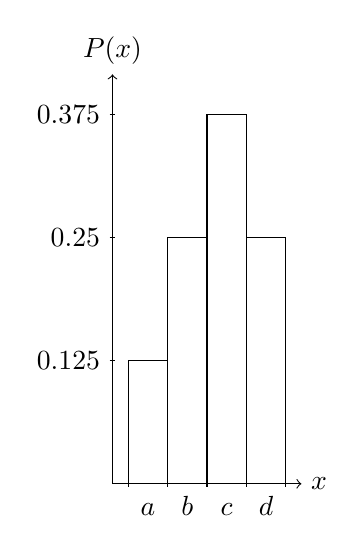
\begin{tikzpicture}
  \drawaxes{P(x)}
  \foreach \y in {0.125, 0.25, 0.375}{
    \draw (-.2cm - 1pt, 12.5 * \y) node[anchor=east] {$\y$}
      --  (-.2cm + 1pt, 12.5 * \y);
  }
  \drawbar{0\barwidth}{0.125}{}
  \drawbar{1\barwidth}{0.25 }{}
  \drawbar{2\barwidth}{0.375}{}
  \drawbar{3\barwidth}{0.25 }{}
\end{tikzpicture}
}

\newcommand{\drawapprox}[2]{
\begin{tikzpicture}
  \tikzmath{
    \splus = #1 + 1;
    \yunit = 12.5 / \splus;
  }
  \draw[xstep=\barwidth, ystep=\yunit, lightgray, very thin]
    (0, 0) grid (4 * \barwidth, 5.2);
    \drawaxes{s'}
  \foreach \y [parse=true, count=\s] in {\yunit, 2 * \yunit, ..., 5.2}{
    \node (tick) at (-.2cm, \y) {};
    \draw ($(tick) - (1pt, 0)$) -- ($(tick) + (1pt, 0)$);
    \draw ($(tick) - (0, \yunit / 2) - (.05, 0)$) node[anchor=east]
      {\pgfmathparse{int(\s - 1)} #2 $\pgfmathresult$};
  }
  \foreach \x/\freq/\start in {0/1/0, 1/2/1, 2/3/3, 3/2/6}{
    \foreach \y [parse=true, count=\s] in {\yunit, 2 * \yunit, ..., 5.2}{
      \tikzmath{
        \snew = int(8 * int((\s - 1) / \freq) + mod((\s - 1), \freq) + \start);
        if \snew>#1 then {\toprint = \snew;} else {let \toprint = ;};
        }
      \draw ($6.25/\splus*(0, -1) + 0.45*(\barwidth,0)
      + \s*(0, 12.5 / \splus) + \x*(\barwidth, 0)$)
      node [text=lightgray] {#2 $\toprint$};
    }
  }
  \drawbar{0\barwidth}{0.125}{thin, gray}
  \drawbar{1\barwidth}{0.25} {thin, gray}
  \drawbar{2\barwidth}{0.375}{thin, gray}
  \drawbar{3\barwidth}{0.25} {thin, gray}
  \foreach \x/\freq/\start in {0/1/0, 1/2/1, 2/3/3, 3/2/6}{
    \foreach \y [parse=true, count=\s] in {\yunit, 2 * \yunit, ..., 5.2}{
      \tikzmath{
        \snew = int(8 * int((\s - 1) / \freq) + mod((\s - 1), \freq) + \start);
        if \snew<=#1 then {\toprint = \snew;} else {let \toprint = ;};
        }
      \draw ($(0, -\yunit / 2) + 0.47*(\barwidth,0)
      + \s*(0, \yunit) + \x*(\barwidth, 0)$) node {#2 $\mathbf\toprint$};
    }
  }
\end{tikzpicture}
}

\newlength{\intervalwidth}
\setlength{\intervalwidth}{0.7\textwidth}

\newlength{\gap}
\setlength{\gap}{0.15cm}

\newlength{\lineheight}
\setlength{\lineheight}{0.45cm}
\newcommand{\drawinterval}{
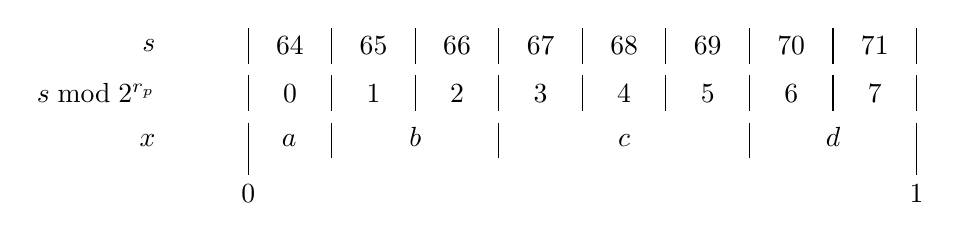
\begin{tikzpicture}
  \draw (-30pt, 0) node [anchor=east] {$s$};
  \draw (0, -.5\lineheight) -- (0, .5\lineheight);
  \draw (\intervalwidth, -.5\lineheight) -- (\intervalwidth, .5\lineheight);
  \foreach \s in {1, ..., 7}{
    \draw (\s * 0.125 * \intervalwidth, -.5\lineheight)
      -- (\s * 0.125 * \intervalwidth, .5\lineheight);
  }
  \foreach \y in {0, ..., 7}{
    \tikzmath{
      \x = (\y * 0.125 + 0.0625);
      \r = int(\y + 64);
    }
    \draw (\x\intervalwidth, 0) node {$\r$};
  }

  \draw (-30pt, -\lineheight -\gap) node [anchor=east] {$s \bmod 2^{r_p}$};
  \draw (0, -.5\lineheight - \gap) -- (0, -1.5\lineheight -\gap);
  \draw (\intervalwidth, -.5\lineheight - \gap)
    -- (\intervalwidth, -1.5\lineheight - \gap);
  \foreach \s in {1, ..., 7}{
    \draw (\s * 0.125 * \intervalwidth, -.5\lineheight - \gap)
      -- (\s * 0.125 * \intervalwidth, -1.5\lineheight - \gap);
  }
  \foreach \s in {0, ..., 7}{
    \tikzmath{
      \x = (\s * 0.125 + 0.0625);
    }
    \draw (\x\intervalwidth, -\lineheight - \gap) node  {$\s$};
  }

  \draw (-30pt, -2\gap - 2\lineheight) node [anchor=east] {$x$};
  \draw (0, -2\gap - 1.5\lineheight) -- (0, -2\gap - 2.5\lineheight - 6pt);
  \draw (\intervalwidth, -2\gap - 1.5\lineheight)
    -- (\intervalwidth, -2\gap - 2.5\lineheight - 6pt);
  \draw (0, -2\gap - 2.5\lineheight - 6pt) node [anchor=north] {$0$};
  \draw (\intervalwidth, -2\gap - 2.5\lineheight - 6pt) node [anchor=north] {$1$};
  \draw (0.125  \intervalwidth, -2\gap - 1.5\lineheight)
    -- (0.125 * \intervalwidth, -2\gap - 2.5\lineheight);
  \draw (0.375  \intervalwidth, -2\gap - 1.5\lineheight)
    -- (0.375 * \intervalwidth, -2\gap - 2.5\lineheight);
  \draw (0.75  \intervalwidth, -2\gap - 1.5\lineheight)
    -- (0.75 * \intervalwidth, -2\gap - 2.5\lineheight);
  \draw (0.06125\intervalwidth, -2\gap - 2\lineheight)
    node [text height=1ex] {$a$};
  \draw (0.25   \intervalwidth, -2\gap - 2\lineheight)
    node [text height=1ex] {$b$};
  \draw (0.5625 \intervalwidth, -2\gap - 2\lineheight)
    node [text height=1ex] {$c$};
  \draw (0.875  \intervalwidth, -2\gap - 2\lineheight)
    node [text height=1ex] {$d$};

\end{tikzpicture}
}
